\documentclass[a4paper,12pt]{article}


\usepackage{./SCUformat}
\usepackage{./cover}

\newcommand{\customtitle}{
    \begin{center}
        \Huge{hello \LaTeX}
        \vspace*{3cm}
    \end{center}
}


\begin{document}

\title{基于人工智能的AI}
\author{郑仕博}
% \authorEng{David Wang}
\adviser{杨波}
% \adviserEng{My Teacher}
\college{计算机学院}
% \collegeEng{Software College}
\major{计算机科学与技术}
% \majorEng{Software Engineering}
\date{\today}
\makecover

\tableofcontents
\clearpage

\section{引言}
\subsection{目的}
本软件设计文档描述了“基于生成式 AI 的个性化文创图像作品设计系统”的
架构与系统设计。面向开发、测试、维护本项目的工程人员及项目管理者,作为
技术实现和系统集成的参考依据。
\subsection{项目范围}
该软件旨在利用生成式 AI 技术解决个性化文创产品供给不足的问题,核心
功能包括:根据用户输入的文本和指定的位置生成创意图像,或编辑现有图像中
的文本。重点目标是实现中文字符的高精度渲染,便于游客与文创从业者快速创
作独特图像作品,助力文旅融合与传播。
\subsection{文档概览}
第 1 章介绍目的、范围、参考资料和术语;第 2 章提供系统概览;第 3 章
详细阐述系统架构;第 4 章描述数据设计;第 5 章介绍各组件设计;第 6 章讲
解人机界面设计;第 7 章为需求矩阵;第 8 章为附录。
\subsection{参考资料}
信息来源于网页\url{https://www.sohu.com/a/823541100_234564}。技术细节参考了
AnyText、TextDiffuser、DDPM 等文献。文档结构基于 IEEE Std 1016-2009 和
上传的 SDD 模板。
\subsection{术语与缩略语}
AI(人工智能)、SDD(软件设计文档)、VAE(变分自编码器)、UNet
(网络结构)、扩散模型、Stable Diffusion(SD)、AnyText(图文生成模型)、
Text-control Diffusion Pipeline 、 Auxiliary Latent Module 、 Text Embedding
Module、Gradio(UI 库)、Prompt(文本提示)、Glyph(字形)、OCR(光
学字符识别)、FID(图像质量指标)、LORA(低秩微调)、CFG-Scale(无
分类引导因子)、eta(扩散采样参数)等术语在文中根据需要进一步解释。

\section{系统概览}
本系统是一个利用生成式 AI 的图像创作工具,支持文本生成图像和图像内
文字编辑,专注于中文字符的精准渲染。系统基于 AnyText 并微调 Stable
Diffusion 模型,通过 Web 界面(Gradio)与用户交互,后端使用 Python 与深
度学习框架实现,支持 Docker 部署。背景需求是解决文创产品同质化问题,赋
能个体创作。

\section{系统架构}
\subsection{架构设计}
系统分为三层:用户界面层(Gradio 实现)、应用逻辑层、核心模型层。
UI 层:负责输入(文本、图像、参数、坐标绘制)与结果展示。
逻辑层:解析输入、格式化参数、调用模型、处理输出与数据管理。
模型层:以 AnyText 为核心,包括三大子模块:
\begin{enumerate}
    \item 文本嵌入模块(Text Embedding Module):处理提示词和字形,生
    成文本语义嵌入;
    \item 辅助潜变量模块(Auxiliary Latent Module):处理位置、掩码等空间
    信息;
    \item 文本控制扩散管道(Text-control Diffusion Pipeline):基于 UNet 模
    型生成图像,受前两模块的条件引导,最终由 VAE 解码生成图像。
\end{enumerate}
\subsection{分解描述}
Text Embedding Module:接收用户提示词和需渲染文本,生成对应
字形图,提取嵌入后送入 Transformer 编码器;

Auxiliary Latent Module:接收坐标、掩码、字形图,通过卷积处理
生成与扩散模型匹配的空间向量;

Diffusion Pipeline:以初始噪声为起点,联合文本嵌入与空间特征逐
步去噪生成图像潜变量,最后 VAE 解码;

Gradio UI:提供文本输入、图像上传、画布交互、参数调节、结果
展示等功能。
\subsection{设计原理}
采用 AnyText + Stable Diffusion 架构,针对中文文本渲染难题,结合字形
信息与位置控制;Realistic\_Vision\_V4.0 作为底模保证图像质量;中文语料微调
提升语义理解;Dreambooth 对文化图像样式微调;Gradio 快速构建 UI。相较
Photoshop、Canva 等工具,该方案更友好、更灵活,适配多语言和编辑需求,
但也需更高计算资源和复杂集成。

\section{数据设计}
\subsection{数据说明}
输入数据包括提示词(文本)、需渲染文本、位置坐标、参考图像(可选)、
控制参数;训练数据包含两类:

AnyWord-3M 标注数据(JSON 格式),用于位置与字符控制训练;

文创图像+文本描述(TXT 格式),用于风格微调。

输出图像保存在服务器(JPG/PNG 格式),模型权重以文件形式存储。
\subsection{数据字典}
user\_prompt:字符串

text\_to\_render:字符串列表

position\_data:坐标列表

edit\_mask:掩码图像/张量

reference\_image:上传图像

control\_params:参数字典,如{'cfg\_scale': 7.5}

generated\_image:最终图像路径或文件

training\_data\_1:AnyWord-3M JSON 结构

training\_data\_2:TXT 列表与对应图像

model\_weights:模型权重文件

glyph\_image、text\_embedding、auxiliary\_latent、image\_latent:中间张
量

hehe98/wenchuang: 项目镜像

wenchuang.ckpt: 模型权重

strength: 文字渲染控制强度,可以为 0 即不使用文字渲染

CFG-Scale: 文字控制强度,低的话会导致生成图像与描述不符合,高的
话图像会不自然

eta:风格多样性,1 表示启用(更具变化),0 不启用(更保守)

\section{组件设计}
主要功能以组件化方式组织,核心函数如下:

generate\_image:解析提示词,生成字形图和文本嵌入,调用辅助模块生成
空间信息,联合生成潜变量图像,再解码输出;

edit\_image:编码参考图像,加入掩码噪声生成初始状态,调用编辑流程生
成新图像并融合原图。

每个过程中的局部变量包括潜变量,预测噪声,注意力图等张量,模块间依
次传递处理。

\section{人机界面设计}
\subsection{界面概览}
提供 Web 端界面,两种主要操作模式:
\begin{enumerate}
    \item 文本生成”:输入提示词与需渲染文本,通过画布绘制或随机选择文本位
    置;
    \item 上传图片,手动掩盖修改区域,输入新文本并生成修改结果。
\end{enumerate}

用户可调整 CFG-Scale、Steps 等参数,查看结果并保存。
\subsection{界面截图}
详情见图1,图2.
\begin{figure}[htbp] % 控制图片浮动位置的选项 (h: here, t: top, b: bottom, p: page)
    \centering % 让图片在页面上居中显示
    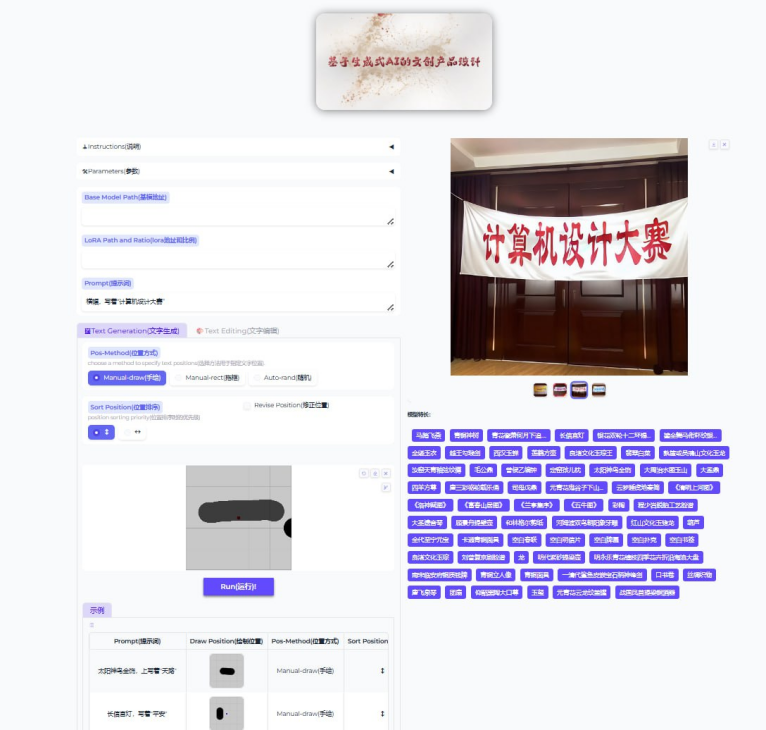
\includegraphics[width=1\textwidth]{Image/UI_1.png} % 插入图片并设置宽度
    \caption{这是图片的标题} % 添加图片标题
    \label{fig:logo} % 添加标签,方便在文中引用,例如 \ref{fig:logo}
\end{figure}
\begin{figure}[htbp] % 控制图片浮动位置的选项 (h: here, t: top, b: bottom, p: page)
    \centering % 让图片在页面上居中显示
    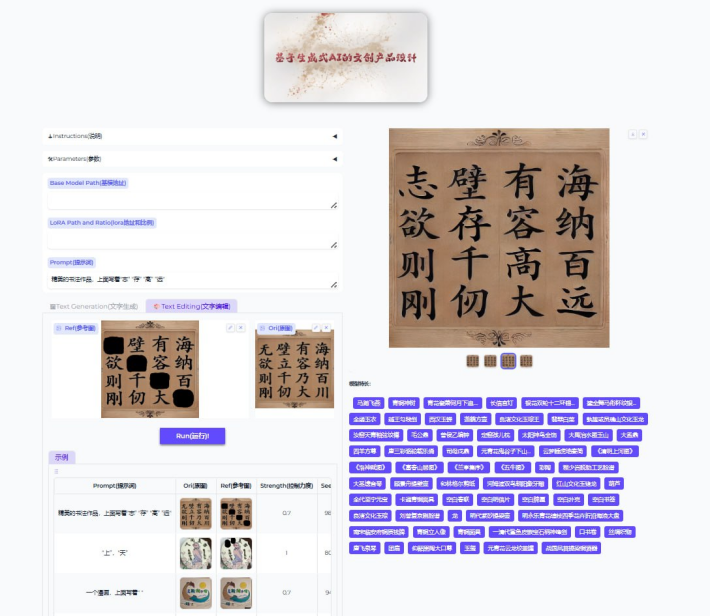
\includegraphics[width=1\textwidth]{Image/UI_2.png} % 插入图片并设置宽度
    \caption{这是图片的标题} % 添加图片标题
    \label{fig:logo} % 添加标签,方便在文中引用,例如 \ref{fig:logo}
\end{figure}

\subsection{界面控件与操作}
\noindent 包括:

文本输入框(Prompt)

位置选择方式(单选按钮)

绘制画布(支持自由绘制、矩形、掩码)

参数调节控件(滑动条/输入框)

“运行”按钮

图像展示区域

上传图片控件

示例加载按钮

参考生成的物品

\noindent 操作:

用户可进行输入、点击、拖动、选择文件等交互。
\section{需求矩阵}
详情见表1。
\begin{table}[htbp] % h: here, t: top, b: bottom, p: page of floats
    \begin{tabular}{|p{0.3\linewidth}|p{0.6\linewidth}|}
        \hline
        \textbf{功能需求} & \textbf{对应组件} \\
        \hline
        文本输入与图像生成 & UI(输入、按钮)、逻辑层、Text Embedding、Aux Latent、Diffusion Pipeline、VAE \\
        \hline
        图像上传与编辑 & UI(上传、掩码、按钮)、逻辑层、VAE 编码、辅助模块、扩散模型、VAE 解码 \\
        \hline
        指定文字位置 & UI(画布、位置选择)、逻辑层、Auxiliary Latent 模块 \\
        \hline
        参数调节 & UI 控件、逻辑层、Diffusion Pipeline \\
        \hline
        结果预览 & UI 显示区、逻辑层 \\
        \hline
        保存分享 & UI 下载、后端文件存储 \\
        \hline
        高中英文渲染准确率 & Text Embedding、Auxiliary Latent、训练数据 1 \\
        \hline
        文化主题生成 & Diffusion Pipeline(微调模型)、训练数据 2 \\
        \hline
        文字图像自然融合 & Diffusion Pipeline、辅助模块、嵌入模块 \\ % Note: "嵌入模块" might refer to Text Embedding
        \hline
        简洁易用界面 & Gradio UI、应用逻辑 \\
        \hline
        示例与指导 & UI 示例加载与静态说明 \\
        \hline
    \end{tabular}
    \centering % Center the table
    \caption{功能需求与对应组件矩阵} % Add a caption
    \label{tab:req_matrix} % Add a label for cross-referencing
\end{table}

\section{APPENDICES}
详见材料中的“项目注意事项”文档。


\end{document}
